\documentclass[12pt,a4paper]{article}
\usepackage[utf8]{inputenc}
\usepackage[russian]{babel}
\usepackage[OT1]{fontenc}
\usepackage{amsmath}
\usepackage{amsfonts}
\usepackage{amssymb}
\usepackage{graphicx}
\graphicspath{{Images/}}
\usepackage[left=2cm,right=2cm,top=2cm,bottom=2cm]{geometry}
\usepackage{calc}
\usepackage{wrapfig}
\usepackage{setspace}
\usepackage{indentfirst}
\usepackage{amssymb}
\usepackage{subfigure}
\usepackage{multirow}

\title{
Отчет о выполнении лабораторной работы 3.4.5

Петля гистерезиса (динамический метод)
}

\author{Комкин Михаил, группа Б01-303}
\newpage
\begin{document}

\maketitle

\textbf{Цель работы:} изучение петель гистерезиса различных ферромагнитных
материалов в переменных полях.

\textbf{В работе используются:} автотрансформатор, понижающий трансформатор, интегрирующая цепочка, амперметр, вольтметр, электронный
осциллограф, делитель напряжения, тороидальные образцы с двумя обмотками.

\section{Теория}
Помимо диа- и парамагнетиков, которые слабо реагируют на внешнее
магнитное поле, в природе существуют вещества, способные сильно намагничиваться даже в небольших полях. Такие вещества относят к классу ферромагнетиков. Это — железо, никель, кобальт, гадолиний
и их многочисленные сплавы. Ферромагнитными свойствами обладают
некоторые сплавы элементов, которые порознь не являются ферромагнитными (например, сплавы меди и марганца), и ряд неметаллических
веществ (ферриты). Ферромагнитные явления сложны и многообразны,
и мы ограничимся изложением лишь некоторых основных фактов.
Зависимость намагниченности $M$ от напряжённости магнитного поля $H$ у всех ферромагнетиков оказывается нелинейной: магнитная восприимчивость $\chi$ не является константой и зависит от $H$. По абсолютной
величине восприимчивость достигает значений $10^3 ÷ 10^4$.
Кроме того, анизотропия кристаллической решётки приводит к тому, что $\chi$ может иметь
тензорный характер (векторы $M$ и $H$ не сонаправлены).
Как и в случае парамагнетиков, атомы ферромагнетика обладают
собственным магнитным моментом. Однако даже в отсутствие внешнего магнитного поля атомы ферромагнетика способны образовывать упорядоченные структуры (домены), в которых все магнитные моменты
ориентированы практически в одном направлении. Таким образом, каждый отдельный атом испытывает влияние не только внешнего поля, но
и поля, созданного коллективом его соседей. \\

\textbf{Модель среднего поля}
В качестве простейшей эмпирической модели, описывающей такую ситуацию, можно рассмотреть следующую
модель: предположим, что намагниченность элемента среды пропорциональна некоторому эффективному полю $H_\text{эфф}$, складывающемуся из
поля $H$ в данной точке, созданного сторонними токами, и среднего «коллективного» поля, пропорционального величине намагниченности $M$:
\[
    M = \chi_\text{пар} H_\text{эфф}
\]
\[
    H_\text{эфф} = H \beta M
\]
где $\chi_\text{пар}$ — парамагнитная восприимчивость отдельного атома, $\beta$ - некоторая безразмерная константа, определяемая из опыта.
Модель среднего поля позволяет уточнить закон Кюри. Определяя
магнитную восприимчивость по-прежнему как $\chi = M/H$, найдём из
(4.9):
\[
\chi = \frac{1}{\chi^{-1}_\text{пар}} \propto \frac{1}{T - \Theta}
\]
где параметр $\Theta = \beta \frac{\mathfrak{m} \mu_0 n}{3k_\text{Б}}$
Соотношение (4.10) называют законом Кюри-Вейсса.

\textbf{Образование доменов}
Остановимся кратко на причине, по которой соседним магнитным моментам выгодно объединяться в домены.
В первую очередь подчеркнём, что магнитное (диполь-дипольное) взаимодействие между атомами не может привести к упорядочению системы. Чтобы в этом убедиться, достаточно оценить энергию такого взаимодействия: из квантовой механики известно, что магнитный момент
атома по порядку величины равен $\mathfrak{m}_\text{Б} = 9,3 \dot 10-24$ Дж/Тл (магнетон
Бора), характерное расстояние между атомами $a \sim 2 \cdot 10^{-10}$ м, тогда
характерное межатомное магнитное поле $B \sim \mu_0 \frac{\mathfrak{m}_\text{Б}}{a^3} \ sim 1$ Тл, 
и характерная энергия диполь-дипольного взаимодействия $U_\text{дип} \sim \mathfrak{m}_\text{Б} B \sim 10^{-4} $эВ.
При такой энергии связи тепловое движение обеспечит полное разупорядочение уже при $T \sim 1$К.
Единственное взаимодействие, которое способно выстроить в ряд
магнитные моменты электронов в атомах при температурах порядка
комнатной, — это электростатическое взаимодействие (его энергия на
несколько порядков больше магнитной: $e^2/(4\pi \varepsilon_0 a) \sim 1$ эВ). Как следует
из квантовой механики, если магнитные моменты (или спины) электронов соседних атомов сонаправлены, их электростатическое отталкивание становится меньше. Таким образом, магнитным моментам атомов энергетически выгодно ориентироваться в одном направлении. Такое явление получило название обменного взаимодействия.

С другой стороны, магнитное дипольдипольное взаимодействие между доменами препятствует выстраиванию всех
магнитных моментов среды в одном направлении. Действительно, энергия такого взаимодействия будет минимальной при антипараллельном расположении магнитных моментов соседних элементов среды. Поэтому при определённом поперечном размере домена оказывается энергетически выгодно иметь соседний домен с противоположно ориентированным моментом (см. рис. 1, слева).
Наложение внешнего поля заставляет домены ориентироваться по нему,
что приводит к резкому увеличению намагниченности образца, а при достаточно большом поле достигается состояние насыщения, когда все
домены ориентируются по полю (см. рис. 1, справа).



\begin{figure}[h!]
    \centering
    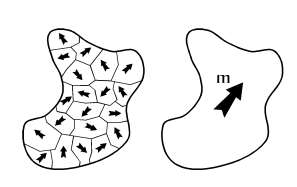
\includegraphics[width=0.6\textwidth]{structure.png}
    \caption{Доменная структура ферромагнетика при слабом (слева) и сильном (справа)
    внешнем поле}
\end{figure}

\textbf{Ферромагнитный гистерезис}
Если состояние некоторой системы зависит не только от мгновенных
значений внешних параметров, но от истории их изменений, говорят, что
в системе имеет место гистерезис.
Именно такими свойствами обладает магнитный момент ферромагнитного образца как функция напряжённости поля $M(H)$. В частности,
система может оказаться намагниченной, даже когда внешнее поле выключено — этим объясняется существование постоянных магнитов. Рассмотрим данное явление подробнее.
Кривая намагничивания. Пусть ферромагнетик находится исходно
в ненамагниченном состоянии ($M = 0$). Медленно увеличивая поле $H$ в
образце, получим зависимость $M(H)$, которую называют начальной кривой намагничивания. Эту кривую обычно разделяют на пять условных
участков (рис. 4.3).
Участок 1 — область обратимого намагничивания, где $M = \chi H$.
В этой области происходят процессы упругого смещения границ доменов: увеличивается размер тех доменов, магнитный момент которых близок к направлению магнитного поля, и уменьшаются размеры доменов
с противоположным направлением магнитного момента.

Участок 2 характеризуется
квадратичной зависимостью $M$
от $H$. В этой области также идёт
процесс обратимого смещения
границ, но проявляется нелинейный характер зависимости
намагниченности от поля.
Область максимальной скорости роста намагниченности 3 соответствует необратимым смещениям стенок между доменами («стенок Блоха»): им приходится преодолевать «препятствия» в виде
примесей, дислокаций и дефектов кристаллической решётки. Когда стенка наталкивается на такое препятствие, она останавливается и держится, пока поле не достигнет порогового значения, при котором она внезапно срывается. Таким образом, движение доменной стенки приобретает
скачкообразный характер («скачки Баркгаузена»).
В достаточно сильных полях движение стенок прекращается, и энергетически выгодным становится поворот магнитных моментов тех оставшихся доменов, у которых магнитный момент не совпадает с направлением поля (область 4).
И, наконец, при некотором значении поля (участок 5) все магнитные
моменты выстраиваются по полю — намагниченность образца достигает
насыщения ($M = M_s$).
На практике магнитные свойства ферромагнетиков обычно изучают
путём измерения зависимости индукции магнитного поля $B$ от напряжённости магнитного поля $H$ в веществе. Исследование образца обычно
начинают с полностью размагниченного состояния ($H = 0, B = 0$). Если
монотонно увеличивать напряжённость $H$, то изменение $B$ происходит
по рассмотренной выше начальной кривой намагничивания с учётом соотношения (4.1): $B(H) = \mu_0(H + M(H))$ (кривая OA на рис. 4.4).
Наклон кривой намагничивания характеризуется дифференциальной магнитной проницаемостью.
\[
\mu_\text{диф} = \frac{1}{\mu_0} \frac{dB}{dH}
\] 

С ростом $H$ величина $\mu_\text{диф}$ сначала растёт (этому соответствуют участки 1 и 2 на рис. 4.3), затем (с середины участка 3) начинает резко падать,
приближаясь к единице при насыщении.
\begin{figure}[h!]
    \centering
    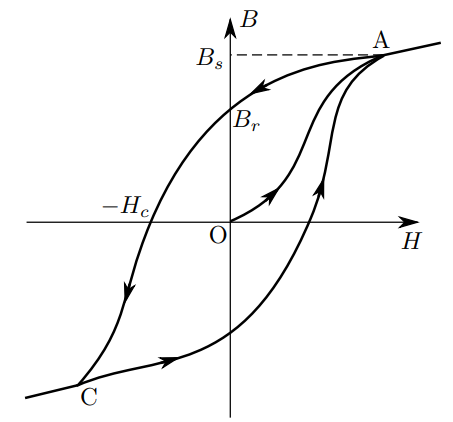
\includegraphics[width=0.6\textwidth]{histeresis_loop_1.png}
    \caption{Петля гистерезиса ферромагнетика}
\end{figure}

\textbf{Явление гистерезиса.}
Доведём систему до некоторой точки $A$, лежащей в области насыщения (здесь $B_s$ — индукция насыщения), и
начнём уменьшать напряжённость $H$. Поскольку между доменами есть
трение, обратный путь пойдёт не по начальной кривой, а выше неё.
При выключения внешних полей, то есть при достижении $H = 0$,
в образце сохраняется некоторое собственное намагничивание. Соответствующее значение индукции $B_r$ называют остаточной индукцией.
Значение $B = 0$ достигается лишь при некотором отрицательном значении $H  = - H_c$. Величина $H_c$ называется коэрцитивным полем. 
В точке С наступает насыщение для намагничивания в противоположную сторону.
Если теперь попробовать вернуться в точку A, вновь наращивая поле, получим некоторый замкнутый цикл (предельную петлю гистерезиса).

Если в точке А насыщение не достигается, то аналогичным
образом получится цикл меньшей площади.
Отметим, что площадь петли гистерезиса ферромагнетика на плоскости H-B есть энергия, необратимо выделяющаяся в виде тепла в еди­нице объёма вещества за один цикл:
\[
\Delta w = - \oint {H dB}
\]
\section{Измерение магнитной индукции}

Ферромагнитные материалы часто применяются в трансформаторах, дросселях, машинах переменного тока, то есть в устройствах, где они подвергаются периодическому перемагничиванию, — поэтому изучение магнитных характеристик ферромагнетиков в переменных полях представляет большой практический интерес. Основные характеристики ферромагнетиков — их коэрцитивное поле $H_c$, магнитная проницаемость $\mu$, рассеиваемая в виде тепла при перемагничивании мощность — зависят от частоты перемагничивающего поля. В данной работе кривые гистерезиса ферромагнитных материалов изучаются в поле частоты $\nu_0 = 50$ Гц с помощью электронного осциллографа.

\begin{figure}[h!]
    \centering
    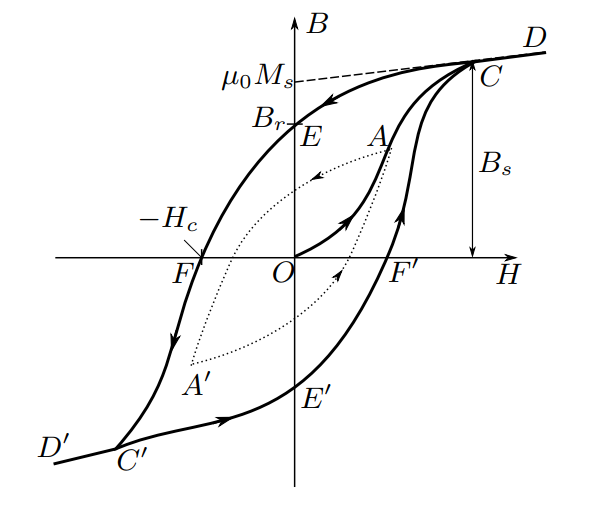
\includegraphics[width=0.6\textwidth]{hysteresis_loop.png}
    \caption{Петля гистерезиса ферромагнетика}
\end{figure}


\subsection{Размагничивающий фактор}

Когда говорят о кривой намагничивания \(B(H)\), речь идёт о локальной связи между индукцией и напряжённостью магнитного поля в каждой точке среды. При этом под \(H\) имеется в виду не только внешнее магнитное поле, а именно поле внутри данного материала. Поскольку непосредственному изменению внешнее поле подвергается внутри образца, изменяемого сторонними токами (в этом образце), необходимо ввести связь между \(H\) и \(H_0\) (внешним, или \(H_0\)).

Для этого вводится векторная величина — размагничивающий фактор. В случае его использования напряжённость \(H\) определяется через разность между внешним полем \(H_0\) и полем намагниченности \(M\), с учетом размагничивающего фактора \(N_{\text{разм}}\). Такое возможно для каждого отдельного элемента среды, имеющего однородную форму и ориентацию по отношению к внешнему полю \(H_0\). Если рассматривать внешнее поле \(H_0\) через поле намагниченности \(M\) и напряжённость \(H\), связь примет вид:

\[
H_{\text{разм}} = H_0 - N_{\text{разм}} M.
\]



Для одного типа образца размагничивающий фактор зависит только от его формы и ориентации. С учётом этого можно убедиться, что величина может меняться в пределах от \(0 \leq N_{\text{разм}} \leq 1\).

Для образца с известным \(N_{\text{разм}}\), изготовленного из материала с постоянной магнитной восприимчивостью, имеем следующее внешнее поле \(H_0\), намагниченность \(M\), и напряжённость:

\[
H_0 = H + NM, \quad M = \chi H, \quad \text{откуда}
\]

\[
M = \frac{\chi H_0}{1 + N_{\text{разм}} \chi}.
\]


Аналитические выражения для \(N_{\text{разм}}\) могут быть получены только для тел простейшей формы. В частности:

\begin{itemize}
    \item бесконечно длинный цилиндр в продольном поле — \(N_{\text{разм}} = 0\), то есть нет размагничивающего эффекта;
    \item цилиндр в поперечном поле — \(N_{\text{разм}} = 1/2\);
    \item сфера — \(N_{\text{разм}} = 1/3\);
    \item тонкий длинный цилиндр или игла в продольном поле — \(N_{\text{разм}} = 1\).
\end{itemize}

Для тел с произвольной формой \(N_{\text{разм}} \ll 1\), и, таким образом, \(H\) или \(H_0\) для длинных тонких игл можно пренебречь.

\textbf{Измерение в тороидальном образце}
В лабораторных условиях для исследования зависимости $B(H)$ ферромагнитных материалов обычно используют образцы тороидальной формы. Если на тор нагнать равномерную намагничивающую обмотку (рис. 4.5), то поле $H$ внутри тора на окружности радиуса $R$ будет пропорционально току $I$ в обмотке, а его величину можно рассчитать по теореме о циркуляции вектора $H$:

\begin{equation}
H = \frac{I N_0}{2 \pi R}, \tag{4.16}
\end{equation}

где $N_0$ — число витков намагничивающей обмотки. Напряженность магнитного поля в тороидальном образце зависит от $R$, поэтому намагниченность образца можно считать однородной при $r \ll R$, где $r$ — радиус сечения тора.

\begin{figure}[h]
    \centering
    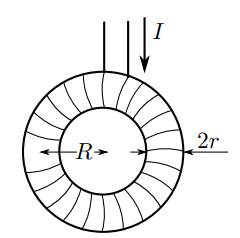
\includegraphics[width=0.3\textwidth]{image.png} 
    \caption{Торроидальный образец с намагниченной обмоткой}
    \label{fig:toroidal_sample}
\end{figure}

\section{Измерение магнитной индукции}

Магнитную индукцию $B$ удобно определять с помощью ЭДС, возникающей при изменении магнитного потока $\Phi$ в катушке, намотанной на образец. Пусть катушка с $N$ витками плотно охватывает образец сечением $S$, и индукция $B$ в образце однородна. Из формулы (4.20) имеем:

\begin{equation}
|B| = \frac{1}{SN} \int E dt.
\end{equation}

Таким образом, для определения $B$ нужно проинтегрировать сигнал, наведённый меняющимся магнитным полем в измерительной катушке, намотанной на образец.

Для интегрирования в работе используется \textit{интегрирующая RC-цепочка} (рис. 2). «Входное» напряжение от источника $U_{\text{вх}}(t)$ подаётся на последовательно соединённые резистор $R_{in}$ и конденсатор $C_{in}$. «Выходное» напряжение $U_{\text{вых}}(t)$ снимается с конденсатора. 

\begin{figure}[h!]
    \centering
    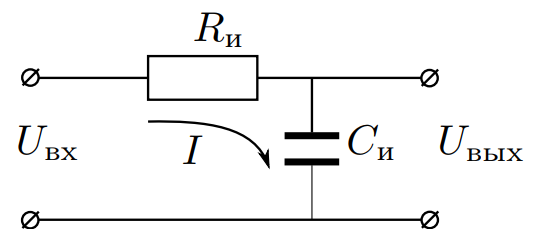
\includegraphics[width=0.4\textwidth]{integrating_circuit.png}
    \caption{Интегрирующая ячейка}
\end{figure}

Предположим, что:

1. Сопротивление источника мало по сравнению с $R_{in}$,
2. Выходное сопротивление осциллографа, равно: $R_{\text{вых}} \gg R_{in}$, 
3. Сопротивление $R_{in}$ достаточно велико, так что почти всё падение напряжения приходится на него, а выходное напряжение близко к $U_{\text{вых}}$.

В таком случае ток цепи равен:

\[
I = \frac{U_{\text{вх}} - U_{\text{вых}}}{R_{in}} \approx \frac{U_{\text{вх}}}{R_{in}},
\]

а входное и выходное напряжения связаны соотношением:

\[
U_{\text{вых}} = \frac{q}{C_{in}} = \frac{1}{C_{in}} \int I dt = \frac{1}{\tau_{in}} \int_0^t U_{\text{вх}} dt,
\]

где $\tau_{in} = R_{in} C_{in}$ — постоянная времени $RC$-цепочки. Для индукции поля из (1) получаем:

\[
|B| = \frac{1}{SN} \int U_{\text{вх}} dt = \frac{\tau_{in}}{SN} U_{\text{вых}}.
\]

\section{Экспериментальная установка}



Схема установки изображена на рис. 3. Напряжение сети (220 В, 50 Гц) с помощью трансформаторного блока $T$, состоящего из регулировочного автотрансформатора и разделительного понижающего трансформатора, подаётся на намагничивающую обмотку $N_0$ исследуемого образца.

\begin{figure}[h!]
    \centering
    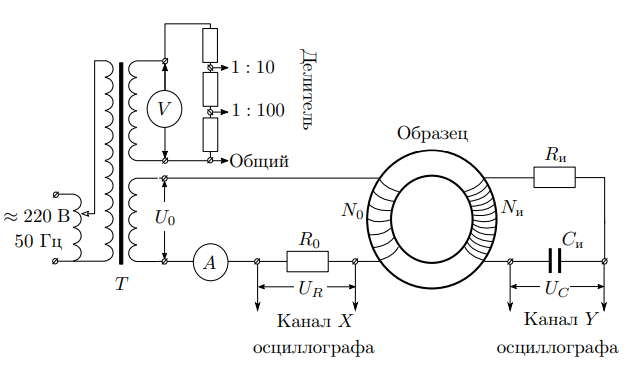
\includegraphics[width=0.7\textwidth]{magnetizing_circuit.png}
    \caption{Схема установки для исследования намагничивания образцов}
\end{figure}

В цепь намагничивающей катушки, на которую подаётся некоторое напряжение $U_0$, последовательно включено сопротивление $R_0$. Напряжение на $R_0$, равное $U_R = R_0 I_0$, где $I_0$ — ток в намагничивающей обмотке $N_0$, подаётся на канал $X$ осциллографа. Связь напряжённости $H$ в образце и тока $I_0$ рассчитывается по теореме о циркуляции (см. (4.16)).

Действующее значение переменного тока в обмотке $N_0$ измеряется амперметром A.
Для измерения магнитной индукции $B$ с измерительной обмотки $N_\text{и}$
на вход RC-цепочки подаётся напряжение $U_\text{и}$ ($U_\text{вх}$), пропорциональное
производной $dB/dt$. С интегрирующей ёмкости $C_\text{и}$ снимается напряжение $U_\text{с}$ ($U_\text{вых}$), пропорциональное величине $B$, и подаётся на вход Y
осциллографа. Значение индукции поля $B$ рассчитывается по формуле (3).
Замкнутая кривая, возникающая на экране, воспроизводит в некотором масштабе (различном для осей X и Y) петлю гистерезиса. Чтобы придать этой кривой количественный смысл, необходимо установить
масштабы изображения, т. е. провести калибровку каналов X и Y осциллографа.



\section{Выполнение}
\textbf{Измерение петли гистерезиса}
\begin{enumerate}
    \item соберем схему представленную на рисунке 6. Подберем ток питания в намагничивающей обмотке, так чтобы на
    экране ЭО наблюдалась предельная петля гистерезиса.
    \item Подберем коэффициенты усиления каналов осциллографа так, чтобы предельная петля занимала большую часть экрана. Зарисуем полученную картину.
    Запишем значения коэффициентов усиления $K_x$ и $K_y$ осциллографа
    и действующее значение тока $I$ в намагничивающей обмотке.
    \item По экрану ЭО измеряем полную ширину и высоту предельной петли ([$2X_s$] и [$2Y_s$]), соответствующие удвоенной амплитуде колебания
    напряжённости $H_s$ и индукции $B_s$ поля в образце в состоянии насыщения. Также измеряем двойные амплитуды для коэрцитивного поля
    [$2X_c$]  и остаточной индукции [$2Y_r$]
    \item Параметры установки $R_\text{и} = 20~\text{кОм}, C_\text{и} = 20~\text{мкФ}, R_0 = 0.22~\text{Ом}$. Параметры образцов:

    \begin{table}[h!]

        \centering
        \begin{tabular}{|c|c|c|c|c|}
          \hline
          Материал     & $N_0$ & $N_\text{и}$ & $S^2$, см$^2$ & $2\pi R$, см \\ \hline
          Феррит       & 40    & 400                              & 3,0           & 25,0         \\ \hline
          Пермаллой    & 20    & 300                              & 0,8           & 13,3         \\ \hline
          Крем. железо & 25    & 250                              & 2,0           & 11,0         \\ \hline
        \end{tabular}
        \caption{Характеристики катушек}
        \label{tab:har_kat}
    \end{table}
      
      


\end{enumerate}
\begin{table}[h!]
    \centering
        \begin{tabular}{|l|l|l|l|l|l|l|}
        \hline 
                          & $K_x$, мВ & $K_y$, мВ & $2X_s$ & $2Y_s$ & $2X_c$ & $2Y_r$   \\ \hline
        Пермаллой         & 20 &         50       &   5.36 &   3.27 &    4.81    & 2.91 \\ \hline
        Феррит            & 5 &          5        &   5.27 &  3.91  &    3.1     & 2.54 \\ \hline
        Кремнистое железо & 50 &         20       &   8.54 &  6.55  &    2       & 4.36 \\ \hline
    \end{tabular}
    \caption{таблица}
\end{table}

\textbf{Калибровка осциллографа} \\ 
Не разбирая схемы «закоротим» намагничивающую обмотку $N_0$.
Измерьте длину наблюдаемой развёртки по оси $X$ при некотором
фиксированном токе $I$, близком к току насыщения петли гистерезиса (осциллограф в режиме $X-Y$ ). Проведите измерения для всех
значений коэффициента усиления $K_x$, использовавшихся в работе.
Учтите, что амперметр измеряет действующее значение тока, меньшее амплитудного в $\sqrt{2}$ раз.
\[
K_X = 2R_0 \sqrt{2} I_\text{эф} /(2x)
\]
\[
K_Y = 2 \sqrt{2} U_\text{эф} /(2y)
\]
\begin{table}[!ht]
    \centering
    \begin{tabular}{|l|l|l|}
    \hline
        $K_x$ & $m_x$ & $\varepsilon$  \\ \hline
        5 & 4.8 & 0.04  \\ \hline
        20 & 19.8 & 0.01  \\ \hline
        50 & 49.5 & 0.01  \\ \hline
        $K_y$ & $m_y$ & $\varepsilon$     \\ \hline
        10 & 9.9 & 0.01  \\ \hline
        20 & 20.8 & 0.04  \\ \hline
        50 & 50.5 & 0.01  \\ \hline
    \end{tabular}
\end{table}
\begin{enumerate}
    \item Измерьте постоянную времени $RC$-ячейки $\tau_{\text{и}}$. Для этого разберем цепь тороида и подадим на вход ячейки синусоидальное напряжение с обмотки $U_0$ понижающего трансформатора.
    Измерьте отношение входного и выходного напряжений $U_{\text{вх}}/U_{\text{вых}}$
    ячейки с помощью осциллографа и/или вольтметра. Рассчитаем постоянную времени по формуле. 
    Частоту сигнала в цепи $\omega_0 = 2\pi \nu_0$
    можно также измерить с помощью осциллографа.
    Сравним результат с расчётом непосредственно через $R_\text{и}$ и $C_\text{и}$, указанные на установке.
    \[
    U_\text{вх} = 5,09 B
    \]
    \[
    U_\text{вых} = 0,04 B 
    \]
    \[
    \tau = RC = U_{\text{вх}}/(\omega U_{\text{вых}})
    \]
    \[
    \tau_{\text{теор}} = 0.4 \text{с}
    \]
    \[
    \tau_{\text{эксп}} = 0.41 \pm 0.06 \text{с}
    \]
    \[
    1/\omega \approx 8 >> \tau
    \]

\end{enumerate}
\[
\varepsilon_{B_s} = \varepsilon_{B_r} = \sqrt{(\varepsilon_{K_y})^2 + (\varepsilon_{2y})^2 }
\]
\[
\varepsilon_{H_s} = \varepsilon_{H_c} = \sqrt{(\varepsilon_{K_x})^2 + (\varepsilon_{2x})^2 }
\]
\begin{table}[h]
    \centering
    \begin{tabular}{|c|c|c|c|}
    \hline
                       &Fe-Ni             & Fe-Si            & Феррит      \\ \hline
    $H$, А/м           & 15.4             & 56.81            & 4.2         \\ \hline
    $B$, Тл            & 0.33             & 0.4              & 0.17        \\ \hline
    $H_{s}$, А/м       & $41\pm 2$        & $186 \pm 7$      & $8.2\pm0.3$       \\ \hline
    $B_s$, Тл          & $0.54 \pm 0.02$  & $1.32 \pm 0.05$              & $0.33\pm 0.01$        \\ \hline
    $H_{c}$, А/м       & $37 \pm 1$        & $56 \pm 2$      & $6.5\pm 0.3$         \\ \hline
    $B_r$, Тл          &$0.48 \pm 0.02$         & $0.87 \pm 0.03$            & $0.21 \pm 0.01$        \\ \hline
    $\mu_{\text{нач}}$, Тлм/A &$(5.5 \pm 0.5) \cdot 10^4$          & $(13.5 \pm 0.6) \cdot 10^4$              & $(3.8\pm 0.2) \cdot 10^4$        \\ \hline
    $\mu_{\text{max}}$, Тлм/A &       $(1.3 \pm 0.1) \cdot 10^5$          & $(10 \pm 1) \cdot 10^5$              & $(1.1\pm 0.1) \cdot 10^5$        \\ \hline
    \end{tabular}
\end{table}
\section*{Вывод}

В данной работе были изучены петли гистерезиса различных ферромагнитных материалов в переменных токах.

Были получены предельные петли и начальные кривые намагничивания для образцов из пермаллоя, феррита и кремнистого железа.  Были рассчитаны цены деления ЭО для петель в $\frac{\text{А}}{\text{м}}$ для оси $X$ и в $\text{Тл}$ для оси $Y$, откуда были найдены коэрцитивная сила $H_c$, индукция насыщения $B_s$ и дифференциальная магнитная проницаемость $\mu_{\text{диф}}$ образцов вблизи нуля. 

\end{document}